%%%%%%%%%%%%%%%%%%%%%%%%%%%%%%%%%%%%%%%%%%%%%%%%%%%%%%%%
%%%%%%%%%%%%%%%%%%%%%%%%%%%%%%%%%%%%%%%%%%%%%%%%%%%%%%%%
\newpage
%\setcounter{section}{0}
\part{Tipos de Datos}
%\begin{center}
%\huge{\textbf{Tipos de Datos}} \\
%\end{center}

En la construcción de algoritmos eficientes, no solo basta la utilización de la lógica correcta para la resolución de problema sino también las estructuras de datos involucradas en dicho algoritmo. Las estructuras de datos están compuestas por  un conjunto de variables que almacenarán los valores necesarios para un algoritmo. Estos valores toman información de acuerdo a un conjunto finito definido por un lenguaje de programación que los identifica. Asociado a estos valores se encuentra una serie de operaciones particulares. A este conjunto de valores y operaciones se le conoce como tipo de dato de un lenguaje de programación.

A continuación estudiaremos en qué consisten los tipos de datos, una pequeña clasificación, que operaciones están asociadas a éstos y cómo están representadas en el computador. 

%%%%%%%%%%%%%%%%%%%%%%%%%%%%%%%%%%%%%%%%%%%%%%%%%%%%%%%%
\section{Definiciones}

Un tipo de dato es un conjunto de valores y un conjunto de operaciones aplicadas a dichos valores en un lenguaje de programación. Dependiendo del lenguaje de programación, un tipo de datos puede ser una estructura de datos, un tipo definido por el programador, un tipo abstracto, una clase, entre otros. Es posible clasificar los tipos de datos en tipos simples o elementales y tipos compuestos o estructurados. En la Fig. \ref{fig:tipodato} se muestra la clasificación empleada de tipos de datos para la notación Alpha empleada.

\begin{figure}[!htb]
\centering
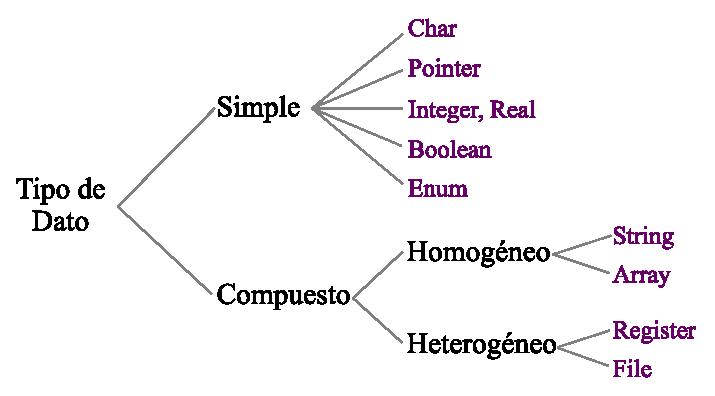
\includegraphics[scale=.7]{images/tipoDeDato.eps}
\caption{Clasificación de los tipos de datos según su naturaleza.}
\label{fig:tipodato}
\end{figure}

El tipo simple está formado por aquellos que no pueden dividirse en componentes, es decir, forman en sí un tipo de dato indivisible o tipo base. Por el contrario, el tipo compuesto está formado por componentes tal que puede descomponerse o dividirse en tipos simples. Entre el tipo simple están el tipo Char, Pointer, Integer, Real, Boolean y Enum. En el tipo compuesto se encuentra el tipo String y Array en una subclasificación de tipo elementos simples de un mismo tipo (homogéneo); y los tipo Register y File que pueden contiener elementos de diversos tipos (heterogéneos).

Es importante destacar que la clasificación se enfoca en los tipos de datos estáticos o creados de forma directa en la mayoría de los lenguajes de programación. Se excluyen tipos compuestos homogéneos dinámicos como listas, árboles, grafos, entre otros.

Básicamente en un lenguaje de programación, es posible expresar los valores de un tipo de dato de 3 formas:
\begin{enumerate}
\item Constantes: denotan un valor en particular dentro del conjunto posible para un tipo de dato.
\item Identificadores, nombres o variables: representan un valor cualquiera del conjunto posible para un tipo de dato asociado a una combinación de caracteres (dependiente del lenguaje).
\item Expresiones: denotan valores como resultado de operaciones entre constantes/identificadores/otras expresiones.
\end{enumerate}

Es importante destacar que cada tipo de dato determina una clase de valores que puede asumir un identificador o expresión las cuales pertenecen a un solo tipo. Por su parte, los operadores actuan sobre operandos de algún tipo y arrojan como resultado algún tipo (que puede ser del mismo tipo o no). Al mismo tiempo, la utilización de los tipos de datos proporciona un ocultamiento de la representación interna en el computador de dichos tipos, ofreciendo una abstracción que es beneficiosa para la portabilidad y semántica de los programas.

Del mismo modo, la verificación de los tipos durante el programa es una tarea importante a realizar. Esta verificación consiste en detectar que cada operación reciba el número adecuado de argumentos y que éstos sean del tipo adecuado. Esto puede ser realizado de forma dinámica o de forma estática, es decir, en momento de ejecución o compilación/traducción respectivamente\footnote{Diferencia entre ensamblador, compilador y traductor}.

A continuación estudiaremos los tipos de datos indicando su organización lógica de definición, así como las operaciones y atributos que posee. También se estudiará la representación que manejan internamente en el computador, la cantidad de memoria que ocupan (CM(tipo)), y el conjunto de valores que puede tomar denominado como cardinalidad (CARD(tipo)).

En este estudio, no se tomará en cuenta el controlador o descriptor que algunos lenguajes de programación asocia a cierto tipos de datos para realizar chequeos de desbordamiento que son ejecutados en tiempo de ejecución. Este descriptor puede incluir identificador únicos que asocian a un identificador así como límites o identificadores de subtipos.

%%%%%%%%%%%%%%%%%%%%%%%%%%%%%%%%%%%%%%%%%%%%%%%%%%%%%%%%
\section{Tipo de Dato Simple}

Los valores de los tipos simples se codifican en la memoria del dispositivo como una secuencia de 0's y 1's. Estos están presente en la mayoría de lenguajes de programación y consideraremos los más esenciales. Por lo general, los tipos de dato simple ocupan lo que se denomina una palabra en memoria, debido a que en el peor de los casos los datos están alineados a frontera de palabra. Una palabra se define como una cantidad de bytes que es dependiente del hardware y está directamente relacionada con el direccionamiento. Por ejemplo, en la tabla \ref{tab:palabra} se muestra el espacio en bytes ocupado para una palabra en diversas arquitecturas.
\begin{center}
\begin{table}[h]
\centering
\begin{tabular}{@{}cc@{}}
\toprule
\multicolumn{1}{l}{Arquitectura} & \multicolumn{1}{l}{Tamaño de la Palabra} \\ \midrule
16 bits                          & 2 bytes                                  \\
32 bits                          & 4 bytes                                  \\
64 bits                          & 8 bytes                                  \\
128 bits                         & 16 bytes                                 \\ \bottomrule
\end{tabular}
\caption{Ejemplo del tamaño de 1 palabra en memoria para diversas arquitecturas.}
\end{table}
\label{tab:palabra}
\end{center}

Se considera que el tamaño de un tipo simple es 1 palabra, es decir, CM(tipo\_simple) = 1. Nótese que las instancias o variables creadas son las que ocupan el espacio en memoria mientras que la representación de los tipos no.

%%%%%%%%%%%%%%%%%%%%%%%%
\subsection{Tipo Integer}

\underline{Conjunto de Valores}: Se define como un subconjunto de $\mathbb{Z}$

\underline{Conjunto de Operaciones}: Suma, resta, multiplicación, división entera (div), residuo (mod), y operaciones relacionales ($>$, $<$, $>=$, $<=$, $==$, $!=$).

En algunos lenguajes existen operaciones bit a bit, es decir, operadores que manejan la representación binaria del tipo Integer tales como desplazamientos/corrimientos de bits o bitwise.

\underline{Representación}: La representación de los enteros se pueden clasificar en enteros sin signo y con signo. Un entero sin signo (unsigned integer) que emplee $n$ bits para su representación, puede representar un total de $2^n$ valores. Po ejemplo, el número decimal 3, en una arquitectura donde el tipo Integer requiera $n=8$ bits, dicho número sería $00000011$.

Por otro lado, un entero con signo (signed integer) requiere que los números negativos sean representado en formato binario. Así, existen diversas representaciones como signo-magnitud, complemento a la base menos uno (o complemento a uno), complemento a la base (o complemento a dos), en exceso a $k$, y base -2. Cada una de las representaciones tiene sus ventajas y desventajas (que no son tema de este curso).

Como ejemplo, se explicará la representación de complemento a dos para el número -6. La forma más sencilla es codificar el número en valor absoluto a su representación en binario, luego invertir todos los bits y finalmente sumarle el valor de 1. Así se tiene:
\begin{lstlisting}[upquote=true,language=pseudo]
00000110 	//representación del número |-6|
11111001	//invertir todos los bits
11111010	//sumarle el valor de 1, entonces 11111010 = -6
\end{lstlisting}

\underline{Cardinalidad}: Dependiendo del número de bits empleados en la representación de un valor tipo Integer, existe una variación en el número de valores posibles que pueden tomar. En la tabla \ref{tab:integer} se muestra el rango de valores y la cantidad de valores para diferentes tamaños de $n$ empleando la representación de complemento a dos.

\begin{center}
\begin{table}[h]
\begin{tabular}{clll}
\hline
\multicolumn{1}{l}{$n$} & Nombre Usual & Rango                                                                                                         & Cardinalidad  \\ \hline
8                              & byte         & \begin{tabular}[c]{@{}l@{}}Con signo: de -8 a 7\\ Sin signo: de 0 a 15\end{tabular}                           & $2^3 - 1$ valores  \\
16                             & short        & \begin{tabular}[c]{@{}l@{}}Con signo: de -128 a 127\\ Sin signo: de 0 a 255\end{tabular}                      & $2^8 - 1$ valores  \\
32                             & int          & \begin{tabular}[c]{@{}l@{}}Con signo: de -2147483648 a 2147483647\\ Sin signo: de 0 a 4294967295\end{tabular} & $2^{32} - 1$ valores \\
64                             & long / int64 & Con signo: de -9223372036854775808 a 9.223372036854775807                                                     & $2^{64} - 1$ valores
\end{tabular}
\caption{Rangos y cardinalidad para algunos valores comunes del tipo Integer empleando $n$ bits.}
\label{tab:integer}
\end{table}
\end{center}

Así, la cardinalidad para el tipo Integer con una representación de $n$ bits es $2^n -1$ valores.

%%%%%%%%%%%%%%%%%%%%%%%%
\subsection{Tipo Real}

\underline{Conjunto de Valores}: Se define como un subconjunto de $\mathbb{R}$

\underline{Conjunto de Operaciones}: Suma, resta,  multiplicación, división, y operaciones relacionales ($>$, $<$, $>=$, $<=$, $==$, $!=$).

Es importante recordar que pueden existir errores en la representación de un número real por truncamiento y redondeo. Así, quizás el siguiente código arroje como salida "Son Distintos":
\begin{lstlisting}[upquote=true, language=pseudo]
Const Real PI = 3.1415926535
if PI == 3.1415926535 then
  Print("Son Iguales")
else
  Print("Son Distintos")
end
\end{lstlisting}

\underline{Representación}: Un número del tipo real es representado con el método de punto flotante el cual es una aproximación de dicho número en el computador. Para ello se requiere de un número fijo llamado parte significativa, y un exponente. Este proceso siempre asumiendo que la base es 2 (base binaria), en ocasiones puede variar a base 10 o 16. Entonces, un número puede ser representado como:

$$parte\_significativa \times base^{exponente}$$

Por ejemplo:

$95.164 = 95164 \times 10^{-2}$

\noindent donde 95164 es la parte significativa, la base es 10, y -2 es el exponente.

Desde hace dos décadas, se emplea en la mayoría de los sistemas computacionales el estándar IEEE 754 para la representación de un número en punto flotante (precisión simple o precisión doble). En dicho estándar, se consideran algunos aspectos para su representación y almacenamiento:
\begin{itemize}
\item Existe un bit de signo, donde 0 representa un número positivo y 1 un número negativo
\item El exponente es base 2
\item Existe un campo de exponente donde se almacena el valor del exponente sumándole el valor de 127 (precisión simple) o 1023 (precisión doble).
\item Se asume que el primer bit de la parte significativa (denominada mantisa) es siempre $1.f$
\end{itemize}

Es importante destacar que el número de bits $n$ empleado depende de la arquitectura del sistema. Brevemente, se muestra el proceso de convertir un número a real a su representación en IEEE 754.

$22,625 (base 10) = 10110,101 (base 2)$

\begin{center}
$(1 \times 2^4) + (0 \times 2^3) + (1 \times 2^2) + (1 \times 2^1) + (0 \times 2^0) + (1 \times 2^{-1}) + (0 \times 2^{-2}) + (1 \times 2^{-3})$
\end{center}

Primero, el proceso consiste es desplazar hacia la izquierda la coma decimal tal que el número se represente de la forma $1.b_1b_2b_3b_4 \dots b_k \times 2^k$, donde $b_1b_2b_3b_4 \dots b_k$ representa a la mantisa y $k$ al exponente. De esta forma queda:

\begin{center}
$1,0110101 \times 2^4$
\end{center}

Por su parte $k=4$, el exponente, pero se almacena sumándole el valor de $127$ (precisión simple), quedando $131$ y su representación en binario es $10000011$. Finalmente, la representación en IEEE 754 de valores de precisión simple es 1 bit para el signo, 8 bits para el exponente y 23 bits para la mantisa. Finalmente, el número 22,625 en binario es:
$$0\mbox{ }10000011\mbox{ }01101010000000000000000$$

La cantidad de memoria que ocupa este tipo es 1 palabra, CM(Integer) = 1 palabra.

\underline{Cardinalidad}: La cardinalidad de un tipo Real con $n$ bits para la parte significativa y $m$ bits para el exponente en representación de complemento a dos se puede calcula como $2^n \times 2^m = 2^{n+m}$. Si la representación es signo-magnitud, existe una doble representación del exponente y parte significativa, por lo que su cardinalidad es $(2^n - 1)\times(2^m - 1)$.

%%%%%%%%%%%%%%%%%%%%%%%%
\subsection{Tipo Char}

\underline{Conjunto de Valores}: El tipo Char es una unidad de información que representa a un símbolo o grafema tal como un alfabeto de una forma escrita. Letras, dígitos numéricos, símbolos de puntuación, espacio en blanco, y otros caracteres pertenecen al conjunto de valores de un tipo Char. Los dos tipos de codificación más empleados son ASCII (American Standard Code for Information Interchange) y UNICODE.

\underline{Conjunto de Operaciones}: Los caracteres pueden verse como un conjunto ordenado sobre el cual pueden realizarse operaciones lógicas y numéricas. Así, es posible aplicar operadores relacionales de acuerdo al código ASCII o UNICODE que representa cada caracter. Por ejemplo, empleando la codificación ASCII, se cumple la siguiente relación:

\begin{lstlisting}[upquote=true, language=pseudo]
97 = 'a' < 'b' < 'c' < ... < 'z' = 122
64 = 'A' < 'B' < 'C' < ... < 'Z' = 122
48 = '0' < '1' < '2' < ... < '9' = 57
\end{lstlisting}

De esta manera, la operación 'a' + 1 == 'b' retornará el valor de true.

\underline{Representación}: La codificación ASCII incluye en su definición 128 caracteres, donde 33 son caracteres de control o no imprimibles y 95 caracteres imprimibles. Para ello solo requiere de 7 bits para almacenar un valor. Actualmente, casi todos los sistemas computacionales emplean el código ASCII o una extensión compatible para textos y para el control de dispositivos que reciben entradas como el teclado. Por ejemplo la codificación UTF-8 (UNICODE Transformation Format) es un formato de codificación orientada a byte (8 bits) que emplea símbolos de longitud variable e incluye la especificación de 7 bits de ASCII. Gran parte de los lenguajes de programación, emplean un byte para representar a un caracter.

Igualmente, la codificación UNICODE incluye codificación con 16 bits de longitud variable (UTF-16) y UTF-32 que es una codificación 32 bits de longitud fija.

La cantidad de memoria que ocupa este tipo es 1 palabra, CM(Char) = 1 palabra.

\underline{Cardinalidad}: De acuerdo al número de bits empleados por cada codificación su cardinalidad varía. Así, si se emplea $n$ bits entonces la cantidad de valores posibles es $2^n - 1$.

%%%%%%%%%%%%%%%%%%%%%%%%
\subsection{Tipo Boolean}

\underline{Conjunto de Valores}: El tipo Boolean tiene dos posible valores (generalmente llamados true y false) que representan los valores de verdad especificados en la álgebra de Boole.

\underline{Conjunto de Operaciones}: Este tipo de dato está asociado principalmente a sentencias condicionales que cambian el control del flujo de ejecución de un programa. Las operaciones algebraicas tales como and, or, == y not son parte del conjunto posible de operaciones que soporta.

\underline{Representación}: Para ello solo bastaría un bit para su representación. Sin embargo, es usual que la unidad mínima de almacenamiento para un tipo de dato sea 1 palabra, por lo que se utiliza 1 palabra para representarlo. Si una palabra se define como 8 bits, entonces se requiere de un byte para su almacenamiento donde el valor de 0 representa a false y 1 a true. Muchas veces, el valor de true se asocia con cualquier valor distinto de 0 (depende del lenguaje de programación).

La cantidad de memoria que ocupa este tipo es 1 palabra, CM(Boolean) = 1 palabra.

\underline{Cardinalidad}: Dado que solo toma dos valores posible, su cardinalidad es 2.

%%%%%%%%%%%%%%%%%%%%%%%%
\subsection{Tipo Enum}

\underline{Conjunto de Valores}: El tipo Enum (también llamado enumerado) es un tipo que consiste en un conjunto de valores llamados elementos, miembros o enumerados del un tipo de dato. Un tipo enumerado está compuesto por valores constantes del lenguaje. Por ejemplo, el tipo Enum llamado suit, contiene dentro de su conjunto a los valores CLUB, DIAMOND, HEART y SPADE. El orden de los valores constantes es importante en la definición de un tipo Enum. Generalmente y por convención, se suelen colocar los elementos con letras mayúsculas.

\underline{Conjunto de Operaciones}: Los operadores aritméticos y relacionales son posibles para cada uno de sus elementos, pero siempre tomando en cuenta que el resultado de la operación se encuentre en el rango definido por el enumerado.

\underline{Representación}: A cada constante del tipo Enum se le asocia un valor entero comenzando desde el 1, y de manera consecutiva para los otros elementos. Por ejemplo, la siguiente definición es correcta (basada en la notación Alpha):
\begin{lstlisting}[upquote=true, language=pseudo]
Type Enum eDir = [NORTH, EAST, SOUTH, WEST]
eDir direction = 2
select
  direction == NORTH: 
    Print ("Hacia el Norte")
    break
  direction == EAST: 
    Print ("Hacia el Este")
    break
  direction == SOUTH: 
    Print ("Hacia el Sur")
    break
  direction == WEST: 
    Print ("Hacia el Oeste")
    break
end
\end{lstlisting}

Nótese que la salida será "Hacia el Este", y dado que es posible asignarle valores del tipo Integer directamente a un tipo Enum, entonces se representa como un valor entero que representa la cantidad de elementos que posee el enumerado. Para el caso del ejemplo, se almacena el valor de 4.

La cantidad de memoria que ocupa este tipo es 1 palabra, CM(Enum) = 1 palabra.

\underline{Cardinalidad}: La cardinalidad se deriva del número de elementos o miembros del tipo Enum.

%%%%%%%%%%%%%%%%%%%%%%%%
\subsection{Tipo Pointer}

Un tipo Pointer se refiere a valores que hacen referencia otro valor almacenado en una posición de memoria. Entonces, este tipo de dato referencia a una dirección de memoria. En la sección \ref{lb:pointer} se hace un estudio detallado de este tipo de dato.

%%%%%%%%%%%%%%%%%%%%%%%%
\subsection{Ejemplo de declaraciones}

En la tabla \ref{tab:palabra} se muestra una comparación en la declaración de los distintos tipo de dato simple.

\begin{center}
\begin{table}[h]
\centering
\begin{tabular}{clll}
\hline
Tipo de Dato & \multicolumn{1}{c}{Notación Alpha}       & \multicolumn{1}{c}{C/C++}             & \multicolumn{1}{c}{Java}                 \\ \hline
Integer      & Integer iValue = 3                       & int iValue = 3;                       & int iValue = 3;                          \\
Real         & Real rValue = 3.14159                    & float rValue = 3.14159;               & float rValue = 3.14159;                  \\
Char         & Char cValue = 'x'                        & char cValue = 'x';                    & char cValue = 'x';                       \\
Boolean      & Boolean bValue = rValue \textless iValue & bool bValue = rValue \textless iValue & boolean bValue = rValue \textless iValue \\
Enum         & Enum eValue = {[}N, S, E, W{]}           & enum eValue \{N, S, E, W\};           & public enum eValue \{N, S, E, W\};       \\
Pointer      & Integer * pValue                         & int * pValue;                         & \multicolumn{1}{c}{N/A}                  \\ \hline
\end{tabular}
\caption{Ejemplo comparativo de algunas definiciones de los tipos simples en la notación Alpha, C/C++ y Java.}
\label{tab:palabra}
\end{table}
\end{center}

En la tabla \ref{tab:palabra} se puede observar que la definición del tipo Pointer (indicando una posición de memoria) no está presente en Java. Igualmente, para ambos lenguajes, solo es un subconjunto posible de definiciones de tipo de dato. Un ejemplo, en el lenguaje Java la definición del tipo Enum solo está presente a partir de la versión 1.5 que data del año 2004.

En en lenguaje C++ existen diversos tipos de datos que varían de acuerdo al número de bits que poseen, o si consideran números con signo y sin signo. Así se pueden definir tipos int, unsigned int, signed int, short int, long int, entre otros. La definición de estos tipos varía de acuerdo al rango que operan y su tamaño depende tanto del compilador que se utiliza así como de la arquitectura del computador.

Empleando C++, es posible conocer el tamaño en bytes de los tipos de datos con la instrucción sizeof. Un ejemplo de ello sería:
\begin{lstlisting}[upquote=true, language=C++]
#include <iostream>
#include <cstdlib>
using namespace std;

int main()
{
   cout << "Size of char: " << sizeof(char) << endl;
   cout << "Size of int: " << sizeof(int) << endl;
   cout << "Size of short int: " << sizeof(short int) << endl;
   cout << "Size of long int: " << sizeof(long int) << endl;
   cout << "Size of float: " << sizeof(float) << endl;
   cout << "Size of double: " << sizeof(double) << endl;
   cout << "Size of wchar_t: " << sizeof(wchar_t) << endl;
   return EXIT_SUCCESS;
}
\end{lstlisting}

Cuando se desea contener una cantidad de tipos de datos considerable o se requiere una estructura más compleja para resolver un problema, se emplean otros tipos de datos: los tipos compuestos.

%%%%%%%%%%%%%%%%%%%%%%%%%%%%%%%%%%%%%%%%%%%%%%%%%%%%%%%%
\section{Tipo de Dato Compuesto}

Como se menciono anteriormente, un tipo compuesto representa a un conjunto de tipos simples que forman al tipo compuesto. Generalmente, un tipo compuesto forma parte de diversos lenguajes de programación como tipo de dato donde cada uno de sus componentes son accedidos. Principalmente se estudiaran los el tipo Array, String, Register y File.

Nótese que tipos homogéneos y de naturaleza dinámica como lo son el tipo List, Queue, Stack, Tree se consideran tipos compuestos.

%%%%%%%%%%%%%%%%%%%%%%%%
\subsection{Tipo Array}

%%%%%%%%%%%%%%%%%%%%%%%%
\subsubsection{Unidimensional}

\underline{Conjunto de Valores}: Valores que pueden ser simples o compuestos de la forma $(e_{li}, e_{li+1}, ..., e_{ls-1}, e_{ls})$, donde $e_i$ es del tipo base del arreglo. Así, el número de valores es $<ls> - <li> + 1$, y sobre cada valor se aplican las mismas operaciones del tipo base del arreglo.

\underline{Operación Constructora}: Es posible definir un arreglo y asignar valores de diversas formas. La primera consiste en crear el arreglo y luego asignar sus valores uno a uno:

\begin{lstlisting}[upquote=true, language=pseudo]
Array aValues of Integer [1..5]
aValues[1] = 1
aValues[2] = 1
aValues[3] = 2
aValues[4] = 3
aValues[5] = 5
\end{lstlisting}

En dicha definición se observa que el número de elementos es $<ls> - <li> + 1 = 5 - 1 = 4$ y que luego de asigna uno a uno sus valores. Por otro lado, se pueden definir los valores del arreglo unidimensional por extensión en el momento de su construcción de la siguiente forma:

\begin{lstlisting}[upquote=true, language=pseudo]
Array aValues of Integer [] = {1, 1, 2, 3, 5}
\end{lstlisting}

No se indica el tamaño del arreglo debido a que la operación constructora permite asignarle directamente los valores y determinar su dimensión.

\underline{Fórmula de Acceso}: La fórmula de acceso consiste en localizar al elemento de la posición $i$ del arreglo $A$ empleando una dirección de memoria base $dirBase$:

$A(i) = dirBase + (i - li) * CM(TBase)$

Con la fórmula de acceso es posible localizar un elemento del arreglo unidimensional con solo la dirección de memoria inicial asumiendo que cada elemento se encuenta contiguo en memoria. De esta forma, solo empleando desplazamientos es posible tener acceso a un elemento. En la Fig. \ref{fig:array} se muestra un ejemplo para el elemento $i$ del arreglo $A(i)$ tal como se mostró en la fórmula anterior.

\begin{figure}[!htb]
\centering
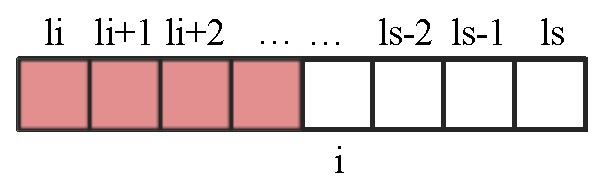
\includegraphics[scale=.7]{images/arreglo.eps}
\caption{La fórmula de acceso permite ubicar el elemento $i$ de un arreglo unidimensional $A$ dada su dirección de memoria base (i.e. la dirección de A[1]) en los límites $li-ls$.}
\label{fig:array}
\end{figure}

\underline{Cardinalidad}: La cardinalidad del tipo Array para el caso unidimensional es $\prod_{i=li}^{ls}{Card(TipoBase)} = Card(TipoBase)^{(ls-li+1)}$

\underline{Cantidad de Memoria}: La cantidad de memoria que ocupa (complejidad en espacio) de un tipo Array unidimensional se define como:

$CM(Array_{1D}) = CM(TipoBase) * (ls - li + 1)$

En algunos lenguajes de programación se suele añadir en el espacio del tipo Array una cabecera o header, también llamado descriptor, que almacena los valores de los límites del arreglo que es de utilidad para el compilador. En los lenguajes modernos, este valor no es empleado porque se definen correctamente lo límites o se calculan en tiempo de ejecución por el compilador.

%%%%%%%%%%%%%%%%%%%%%%%%
\subsubsection{Bidimensional}

\underline{Conjunto de Valores}: Al igual que el tipo Array unidimensional, está formado por tipos simples o compuestos. En este caso, dado que es bidimensional, se requieren los límites tanto para las dos dimensiones: $<li_1, ls_1>$ y $<li_2, ls_2>$

\underline{Operación Constructora}: Un arreglo bidimensional o matriz, se declara básicamente de dos formas:

\begin{lstlisting}[upquote=true, language=pseudo]
Array aMatrix of Integer [1..2][1..3]
aValues[1][1] = 1
aValues[1][2] = 1
aValues[1][3] = 2
aValues[2][1] = 3
aValues[2][2] = 5
aValues[2][3] = 8
\end{lstlisting}

Del mismo modo, se puede crear por extensión los mismo valores:

\begin{lstlisting}[upquote=true, language=pseudo]
Array aMatrix of Integer [][] = {{1, 1, 2}, {3, 5, 8}}
\end{lstlisting}

\underline{Fórmula de Acceso}: La fórmula de acceso consiste en localizar al elemento de la posición $(i,j)$ de la matriz $M$ empleando una dirección de memoria base $dirBase$:

$M(i,j) = dirBase + [(i - li_1)*(ls_2 - li_2 + 1) + (j - li_2)] * CM(TipoBase)$

La Fig. {fig:matrix} muestra un ejemplo para ubicar la posición $(i,j)$ dada la dirección de memoria de inicio de la estructura de datos (i.e. posición $M[1][1]$). La fórmula busca ubicarse $i - li_1$ filas desde la posición inicial, la cantidad del número de filas es $ls_2 - li_2 + 1$. Por último, después de las 3 filas amarillas), se hace un desplazamiento $j - li_2$ más allá del inicio tal como se hace en un arreglo unidimensional.

\begin{figure}[!htb]
\centering
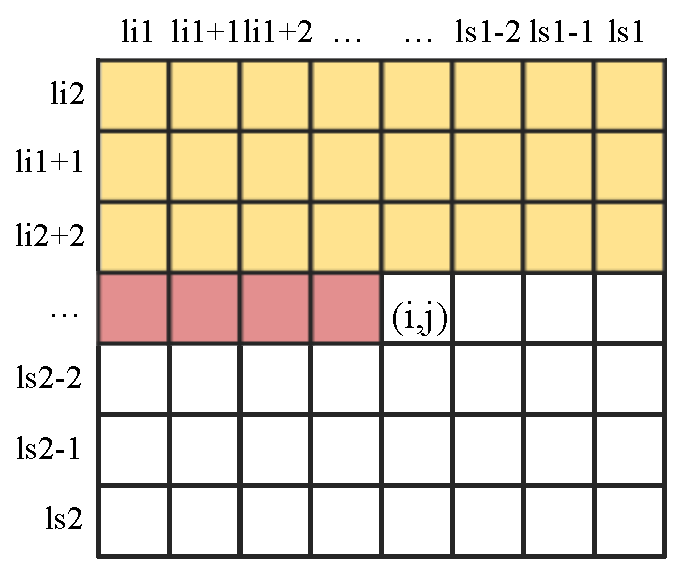
\includegraphics[scale=.7]{images/matriz.eps}
\caption{La fórmula de acceso permite ubicar el elemento $(i,j)$ de una matriz $M$ dada su dirección de memoria base en los límites $li_1,ls_1$ a $li_2,Ls_2$.}
\label{fig:matrix}
\end{figure}

\underline{Cardinalidad}: La cardinalidad para el caso bidimensional es $\prod_{i=li_1}^{ls_1}{\prod_{i=li_2}^{ls_2}{Card(TipoBase)}} = Card(TipoBase)^{(ls_1-li_1+1)*(ls_2-li_2+1)}$

\underline{Cantidad de Memoria}: La cantidad de memoria que ocupa (complejidad en espacio) de un tipo Array bidimensional se define como:

$CM(Array_{2D}) = CM(TipoBase) * (ls_1 - li_1 + 1) * (ls_2 - li_2 + 1)$

Es importante destacar que se asume que la matriz se almacena por filas de forma contigua en memoria. Dependiendo de la arquitectura del computador, los datos de la matriz se pueden almacenar por columnas o por filas.

%%%%%%%%%%%%%%%%%%%%%%%%
\subsection{Tipo String}

\underline{Conjunto de Valores}: El tipo String se puede definir como un arreglo unidimensional de elementos de tipo Char. Por lo que cada valor es un tipo Char, y su longitud viene definido por el máximo a almacenar en dicho tipo. Este valor máximo se define previamente el algoritmo.

\underline{Operación Constructora}: Para definir un tipo String se define una variable de dicho tipo y se le asignan valores literales o de otro identificador del mismo tipo. Es importante destacar que es posible construir un String empleando la operación de sub-string como $[li..ls]$ donde $li$ indica un índice positivo dentro del rango del string y $ls$ un índice positivo dentro del rango tal que $ls \le li$.

\underline{Cardinalidad}: La cardinalidad de este tipo se calcula como el tipo Array con base el tipo Char, es decir Card(Char)$^m$, donde $m = ls - li + 1$ indicando el número de elementos máximos del tipo String.

\underline{Cantidad de Memoria}: La cantidad de memoria que ocupa es simplemente $m$ palabras de memoria.

%%%%%%%%%%%%%%%%%%%%%%%%
\subsection{Tipo Register}

\underline{Conjunto de Valores}: Un tipo Register está formado por valores simples o compuestos $(e_{1}, e_{2}, ..., e_{m-1}, e_{m})$, en donde 

\underline{Operación Constructora}: El tipo Register se define como:

\begin{lstlisting}[upquote=true, language=pseudo]
Register rData
  String sName
  Integer iId
  Char cSex
end
\end{lstlisting}

En el código anterior se declara una variable $rData$ que puede ser empleada en nuestroa algoritmos. Por otro lado, es posible crear un tipo de dato definido por el programador con la instrucción Type como sigue:

\begin{lstlisting}[upquote=true, language=pseudo]
Type Register rtData
  String sName
  Integer iId
  Char cSex
end
rtData oUser1, oUser2
\end{lstlisting}

De esta forma, existe un tipo de dato compuesto heterogéneo rtData y existen dos variables de este tipo llamadas oUser1 y oUser2.

\underline{Operación Selectora}: La operación selectora de un tipo Register es a través del operador punto (.) que permite seleccionar un elemento (simple o compuesto) del registro. Por ejemplo oUser1.sName = "Bart" permite asignarle valores del tipo String al campo sName de la variable oUser1. Es importante notar que también es posible asignar valores al tipo Register sin emplear la operación selectora pero debe ser realizado para todos sus valores:
\begin{lstlisting}[upquote=true, language=pseudo]
rtData oUser1, oUser2
oUser1 = {"Bart", 742, 'M'}
oUser2 = {"Lisa", 741, 'F'}
\end{lstlisting}

\underline{Fórmula de Acceso}: La fórmula de acceso para un campo <identificador>.<campo> del tipo Register, dado su dirección base, se define como:

$dirBase + \sum_{i=1}^{m}{CM(C_i)}$

\noindent donde $m$ es el número de campos del identificador, y $CM(C_i)$ representa la cantidad de memoria que ocupa el campo $k$.

\underline{Cardinalidad}: La cardinalidad de este tipo es:

$Card(Register) = \prod_{i=1}^{m}Card(C_i)$

\underline{Cantidad de Memoria}: La cantidad de memoria que ocupa es la suma de todos los campos que la conforman, $\sum_{i=1}^{m}CM(C_k)$

%%%%%%%%%%%%%%%%%%%%%%%%
\subsection{Tipo File}

El tipo File no será estudiado ya que representa a una estructura que extrae/coloca elementos de archivos y sirve de enlace entre una información estructurada (i.e. en memoria, disco) y el algoritmo.

%%%%%%%%%%%%%%%%%%%%%%%%%%%%%%%%%%%%%%%%%%%%%%%%%%%%%%%%
\section{Tipo de Dato Pointer} \label{lb:pointer}

También llamado apuntador, referencia, puntero o pointer. Una tipo Pointer no es más que un tipo de dato elemental que representa una dirección de memoria en donde por lo general se encuentra un dato, sea simple o compuesto. Los apuntadores son la base para la creación de la mayoría de las estructuras dinámicas, como listas, árboles y grafos. La cantidad de memoria que ocupa cada variable de tipo referencia es 1 palabra. Se declara de la siguiente forma:

\begin{lstlisting}[upquote=true, language=pseudo]
<tipo de dato>* <nombre-variable u objeto>
\end{lstlisting}

Algunos ejemplos:

\begin{lstlisting}[upquote=true, language=pseudo]
Type Register Point
  Real x,y
end
Integer* pInt		// variable apuntador a entero
Point* pPoint		// variable apuntador al tipo Point
Type Point* PPoint	// esto es un tipo apuntador a Point
PPoint pMyPointer	// variable apuntador a Point
\end{lstlisting}

%%%%%%%%%%%%%%%%%%%%%%%%%%%%%
\subsection{Conjunto de valores}

Los valores asociados al tipo referencia son direcciones de memoria. Si se pueden direccionar 4 GB, entonces las direcciones van desde la posición de memoria $0$ hasta $2^{32}-1$ (haciendo abstracción de los mecanismos de direccionamiento). Esto va a depender del tamaño de la dirección en una arquitectura dada. La dirección 0 por lo general está reservada, y se utiliza para inicializar los apuntadores, o indicar que no están apuntando a ningún valor. La constante $NULL$ o $NIL$ es empleada para darle mayor legibilidad a los algoritmos, y no se debe acceder a esta dirección que generalmente es la dirección $0$.

%%%%%%%%%%%%%%%%%%%%%%%%%%%%%
\subsection{Conjunto de operaciones}

Las operaciones más comunes son la asignación y las relacionales. Por lo general sólo interesa comparaciones de igualdad y diferente; raramente se requiere comparar ($>$ o $<$) una dirección con otra. Algunos lenguajes soportan aritmética de punteros donde es posible incrementar o decrementar una dirección. En el caso de la asignación, es importante que ambas direcciones apunten a elementos de un mismo tipo, pues de lo contrario se podrían acceder e interpretar datos de manera errónea. Dos apuntadores son iguales si almacenan la misma dirección de memoria.

Otro operador es la derreferenciación. Este operador retorna el dato referenciado por el apuntador, y se coloca antes del identificador que se desea derreferenciar. Se empleará el símbolo $*$ para derreferenciar y se acostumbra colocarlo entre paréntesis junto con el identificador para mayor legibilidad. A continuación se muestra un ejemplo como continuación del segmento de código anterior:

\begin{lstlisting}[upquote=true, language=pseudo]
pPoint = new Point; //la instrucción new se explica más adelante
*pPoint.x = 0	// se accede la coordenada x del punto pPoint, también se puede emplear como (*pPoint).x
Point ptNew	// se define una variable de tipo registro Point
ptNew = *pPoint	// el punto apuntado por pPoint es asignado a ptNew
\end{lstlisting}

La operación contraria a la derreferenciación es la referenciación (también llamada indirección). Este operador retorna la dirección de una variable u objeto. Se debe emplear mediante la palabra $ref$.

\begin{lstlisting}[upquote=true, language=pseudo]
Point ptMyPoint;
Point * pPointer;
pPointer = ref ptMyPoint;		//pPointer toma la dirección en donde está almacenado  ptMyPoint
*pPointer.x = 4				// se asigna 4 al campo x de pPointer. Equivale a ptMyPoint.x = 4;
*(ref ptMyPoint).y = 3		// solo a manera de ejemplo. Equivale a ptMyPoint.y = 3;
*(*(ref pPointer)).y = 1		// solo a manera de ejemplo. Equivale a ptMyPoint.y = 1;
\end{lstlisting}

El operador $*$ tiene prioridad sobre el operador punto $.$ utilizado para acceder miembros de registros y objetos, y éste sobre el operador $ref$. Entre otros operadores sobre apuntadores se encuentra el $new$ y $delete$.

%%%%%%%%%%%%%%%%%%%
\subsubsection{Operador new}

Este operador reserva el espacio en memoria suficiente para el tipo de dato especificado como parámetro y retorna la dirección de memoria que hace referencia a dicho espacio. Si no se logró reservar el espacio entonces retorna $NIL$. Es buena práctica de programación, verificar que se reservó la cantidad de memoria solicitada. En los compiladores actuales, si no hay memoria, se genera una excepción. En estos casos, hay que manejar las excepciones, y no el valor de retorno. Unos ejemplos de su sintaxis se muestra a continuación:
\begin{lstlisting}[upquote=true, language=pseudo]
Char* pChar = new Char
User* oUser = new User("Homer")
Real** pDoubleReal = new Real*
\end{lstlisting}

Entonces, el operador new reserva el espacio en memoria para el tipo de dato que se está creando. Veamos un ejemplo más extenso:

Ejemplos:
\begin{lstlisting}[upquote=true, language=pseudo]
Integer* pInt
Point* pp

pInt = new Integer	//se asume que siempre se podrá reservar memoria
pp = new Point
*pp.x = 4; *pp.y = 6;
*pInt = 100
\end{lstlisting}

Una posible representación del código anterior se puede observar en la Fig. \ref{fig:pointer} donde se muestra que tanto la variable pInt y pp ocupan un espacio de memoria pero almacenan la dirección, apuntan a, o guardan la referencia de la dirección de memoria de los datos 100 y (4,6) respectivamente.

\begin{figure}[!htb]
\centering
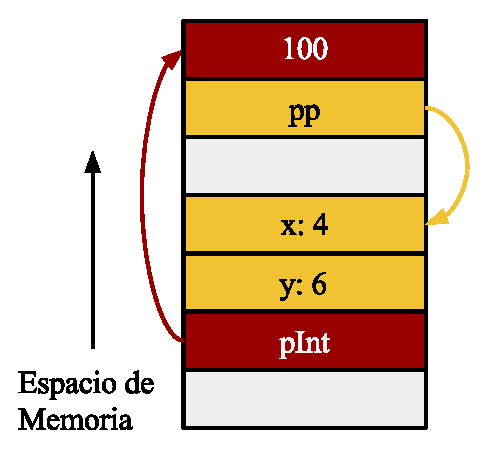
\includegraphics[scale=.7]{images/pointers.eps}
\caption{Ejemplo de representación en memoria del resultado del código anterior empleando punteros.}
\label{fig:pointer}
\end{figure}

%%%%%%%%%%%%%%%%%%%
\subsubsection{Operador delete}

Este operador libera la memoria dinámica reservada mediante el operador new. En su sintaxis, se debe colocar la palabra delete seguido del apuntador a ser borrado.

Como efecto de la operación, o estado final, la memoria es liberada y está disponible para alojar nuevos datos, pero por estar libre, no puede ser accedida, pues generaría un fallo de protección de memoria, por ejemplo:

Ejemplos:
\begin{lstlisting}[upquote=true, language=pseudo]
  delete pInt	// se libera el entero apuntado por pInt
  *pInt = 7	// fallo de protección de memoria
\end{lstlisting}

A pesar que la variable pInt sigue apuntando a la misma dirección de memoria luego del delete, ya esa posición de memoria no le pertenece al espacio de acceso permitido por el programa, y no puede ser accedida ni modificada. Para el caso de apuntadores a objetos, el operador delete invoca al destructor del objeto, y libera el espacio asignado;:

\begin{lstlisting}[upquote=true, language=pseudo]
User oUser = new User ()	
delete oUser		// se invoca al método destructor de User
\end{lstlisting}

En caso que User contenga a su vez atributos de tipo apuntador que hayan solicitado memoria dinámica, estos deben ser liberados en el destructor de la clase User. El operador delete genera un error si la dirección no contiene un dato creado dinámicamente con new, si el dato apuntado ya fue liberado previamente, o si la dirección es NIL.

Los datos que fueron creados con el operador new deben ser destruidos con el operador delete. De lo contrario, ese espacio queda ocupando espacio en memoria hasta que el programa termine su ejecución. Lenguajes como Java y C\# destruyen los objetos automáticamente cuando dejan de ser referenciados, es decir, cuando los apuntadores a esas áreas han desaparecido del ambiente de referenciación. En el caso de C++, se debe invocar explícitamente al operador delete para liberar la memoria (con excepción de los smart pointer).

%%%%%%%%%%%%%%%%%%%
\subsubsection{Memoria Dinámica}

Un apuntador es un número que representa una dirección, y al igual que el tipo Integer ocupa una palabra de memoria. Su cardinalidad es la cantidad de memoria asignable. Actualmente, la cantidad de memoria asignable no es únicamente la cantidad de memoria debido a muchos sistemas soportan el concepto de memoria virtual.

Entre las ventajas en la creación de memoria de forma dinámica está la de reservar espacio para $n$ componentes de un mismo tipo de dato. De esta forma, es posible construir un conjunto de datos de un mismo tipo como un arreglo. El siguiente código permite crear un arreglo de forma estática y dinámica o en tiempo de ejecución.

\begin{lstlisting}[upquote=true, language=pseudo]
Array aArray of Real [1..67]
aArray[5] = 6
Real* prArray = new Real[1..67]
*(prArray + 5) = 6.5  	//es equivalente a utilizar prArray[5] = 6.5
\end{lstlisting}

Se puede observar que para el caso del apuntador prArray, dado que es una dirección de memoria, se puede aplicar la operación de suma a la dirección base de dicho arreglo en 5 posiciones. El resultado es equivalente a aplicar prArray[5], la cual representa una forma más simple de utilizarla.

Dada que la posición del apuntador se encuenta en la primera posición de los datos (que estan continuos en memoria) es posible asignarle un valor a la primera posición de la siguiente forma:

\begin{lstlisting}[upquote=true, language=pseudo]
*prArray = 2.8
\end{lstlisting}

Sin embargo, luego de dicho entero se encuentran 66 datos del tipo Integer más, que pueden ser accedidos derreferenciando una posición de memoria o de forma convencional con el operador selector [].

Dada la diferencia entre aArray y prArray, una definida en tiempo de compilación y la otra en ejecución respectivamente, se debe tomar en cuenta que el espacio solicitado dinámicamente por prArray debe ser liberado. No basta el operador delete en su forma convencional puesto que liberaría sólo el primer elemento. Hace falta indicar que el apuntador referencie a una serie de elementos. De esta manera, se debe emplear la siguiente instrucción:

\begin{lstlisting}[upquote=true, language=pseudo]
delete [] prArray
\end{lstlisting}

Este operador libera todos los elementos que estén alojados desde la posición apuntada por prArray. Si el contenido del arreglo son objetos, entonces se invocará a los destructores correspondientes. Igualmente, cuando se desea crear un arreglo de objetos dinámicamente, sólo puede invocarse al constructor por defecto de los objetos.

Dicho esquema puede aplicarse a arreglos bidimensionales. Un ejemplo para la construcción de una matriz dinámica de $m \times n$ posiciones donde primero se debe construir un arreglo de $m$ posiciones que contenga a apuntadores del tipo base del arreglo. Luego, cada posición almacenará una fila completa del arreglo bidimensional. En este punto, $n$ indica el número de columnas en cada fila del arreglo. En la Fig. \ref{fig:pointer1} se muestra un ejemplo para un arreglo del tipo Integer con $m=4$ y $n=6$.

\begin{figure}[!htb]
\centering
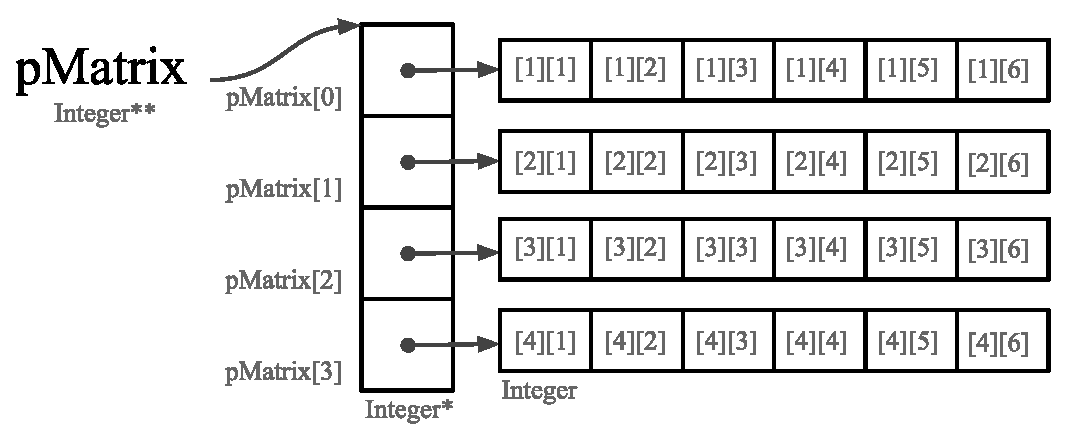
\includegraphics[scale=.65]{images/pointer1.eps}
\caption{Ejemplo de construcción de un arreglo bidimensional de $4 \times 6$ empleando la variable pMatrix.}
\label{fig:pointer1}
\end{figure}

Escribiendo el código, la construcción de la matriz de $4 \times 6$ del tipo Integer empleando memoria dinámica con el apuntador pMatrix queda como:

\begin{lstlisting}[upquote=true, language=pseudo]
Const Integer m = 4
Const Integer n = 6
Integer** pMatrix
Integer iK
pMatrix = new Integer* [m]
for iK = 1 to m do
  pMatrix[ik] = new Integer [n]
end
\end{lstlisting}

Como se observa, se aloja memoria para una alojar apuntadores a las filas para luego,  crear dichas filas de forma dinamica del tamaño de las columnas. Ahora, el proceso para liberar dicha memoria consiste en liberar el espacio de cada fila completa y luego a los punteros de dichas filas. El código asociado para liberar el espacio de la variable de arreglo bidimensional pMatrix es:

\begin{lstlisting}[upquote=true, language=pseudo]
for iK = 1 to m do
  delete [] pMatrix[iK]
end
delete [] pMatrix
\end{lstlisting}

Es posible crear dinámicamente un número distinto de columnas para cada fila, pero esto no entraría en la definición de arreglo. Sin embargo, esta sería una buena forma de definir una estructura de datos llamada Sparse Matrix (ver \ref{sec:sparse} para mayor detalle)

%%%%%%%%%%%%%%%%%%%%%%%%%%%%%%%%%%%%%%%%%%%%%%%%%%%%%%%%
\section{Ideas Finales}

\begin{itemize}
\item El uso de tipos de datos incrementa la legibilidad y semántica de un programa
\item Básicamente, se puede clasificar los tipos de datos por la naturaleza de los valores que almacena (simple o compuesto) o por la forma como son creados (estático o dinámico)
\item La cantidad de memoria de un tipo, llamado complejidad en memoria o espacio que ocupa, corresponde al número de bytes o palabras en memoria que se requiere para su almacenamiento
\item Cualquier función recursiva puede ser sustituida por una equivalente iterativa
\end{itemize}

%%%%%%%%%%%%%%%%%%%%%%%%%%%%%%%%%%%%%%%%%%%%%%%%%%%%%%%%
\section{Problemas}

\begin{itemize}
\item Diseñe una estructura de datos que permita almacenar eficientemente matrices en forma de la letra Z, es decir, matrices con elementos significativos en la diagonal de izquierda a derecha desde arriba a abajo, y en la primera y última fila (con elementos no significativos en el resto). Calcule su costo de memoria, explique por qué es eficiente en comparación con la representación típica, su cardinalidad, la fórmula de acceso para un elemento (i,j) y por último elabora un algoritmo que permita sumar y multiplicar dichas matrices.
\item Asumiendo que todas las variables están contiguas en memoria en el orden que son declaradas, calcule la fórmula de acceso a Total[i].A[j], Total[i].x, y Total[i].y dada la dirección base de Secret y la siguiente definición:
\begin{lstlisting}[upquote=true, language=pseudo]
Type Register Secret
  Char c
  Integer x
  Real y
  Array A of Integer[1..10]
end
Array Total of Secret[-2..-1]
\end{lstlisting}
\item Empleando la definición del tipo Secret (del problema anterior) y con esta definición:
\begin{lstlisting}[upquote=true, language=pseudo]
Type Array CICPC of Secret[1..2]
Type Register Sol
  Array B of CICPC [-2..3]
  Boolean bUnBit
end
Array Moon of Sol [1..10]
\end{lstlisting}
Calcule el espacio o cantidad de memoria de la variable Moon.
\item Escribir la fórmula de acceso k-Dimensional para una matriz de $k$ dimensiones.
\item Considere las siguientes definiciones de tipo:
\begin{lstlisting}[upquote=true, language=pseudo]
Type Array Arr of Integer [-5..5]
Type Array Sub of Arr [-2..6]
Sub Aux
\end{lstlisting}
\begin{enumerate}
\item Indique el costo en memoria de la variable Aux
\item Indique la cardinalidad del tipo Sub
\item Indique la fórmula de acceso de Aux[i]
\item Indique la fórmula de acceso de Aux[i][j]
\end{enumerate}
\item Defina una estructura de datos que permita almacenar eventos de un calendario para fechas válidas. Calcule su cardinalidad, complejidad en espacio, y fórmula de acceso para conocer el evento que se encuentra registrado en cuentro día del año. Asuma que solo se representa un solo año.
\end{itemize}



